\chapter{BACKGROUND} \label{chap:Background}
\section{Notation}

\begin{definition} \label{tensor_indexing}
\noindent For a tensor of rank 3 $\tensor{A}$, let $\tensor{A}_{i,j,k}$ denote the element at the $i$-th page, $j$-th row, and $k$-th column.

\begin{figure}[H]
    \centering
    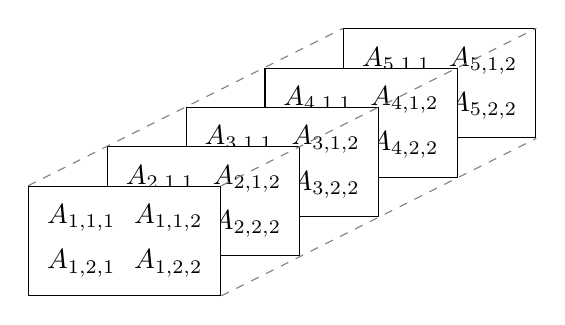
\begin{tikzpicture}
\def\xs{1} %shift in x direction
\def\ys{0.5} %shift in y direction
\def\nm{5} % number of 2d matrices in the 3d matrix
\foreach \x in {5, 4, 3, 2, 1}
{

\matrix [draw, % for the rectangle border
         fill=white, % so that it is not transparent
         ampersand replacement=\&] %see explanation
(mm\x)%give the matrix a name
at(\x * \xs, \x * \ys) %shift the matrix
{

    \node {$\tensor{A}_{\x,1,1}$}; \& \node {{$\tensor{A}_{\x,1,2}$}} ; \\
    \node {{$\tensor{A}_{\x,2,1}$}}; \& \node {{$\tensor{A}_{\x,2,2}$}};\\
};
}
\draw [dashed,gray](mm1.north west) -- (mm\nm.north west);
\draw [dashed,gray](mm1.north east) -- (mm\nm.north east);
\draw [dashed,gray](mm1.south east) -- (mm\nm.south east);
\end{tikzpicture}
\end{figure}
\end{definition}

\begin{definition} \label{matrix_derivative}
Let $\mathbf{A} \in \mathbb{R}^{m \times n}$ and $\mathbf{\x} \in \mathbb{R}^{p \times 1}$. $\tensor{B} = \frac{\partial}{\partial \x}\mathbf{A} \in \mathbb{R}^{p \times m \times n }$ such that
\begin{align*}
    \tensor{B}_{i, j, k} = \frac{\partial}{\partial \x_i}\mathbf{A}_{j, k}
\end{align*}
\end{definition}

\begin{definition}
Let $\S{\mathbf{v}} : \mathbb{R}^{3} \rightarrow \mathbb{R}^{3 \times n}$  denote the skew symmetric cross product matrix of $\mathbf{v}$ \textbf{s.t}
\begin{align*}
    \S{\mathbf{v}} = \begin{bmatrix}
    0 & -\mathbf{v}_2 & \mathbf{v}_1 \\
    \mathbf{v}_2 & 0 & -\mathbf{v}_0 \\
    -\mathbf{v}_1 & \mathbf{v}_0 & 0
    \end{bmatrix}
\end{align*}
\end{definition}


\begin{definition}
Let $\Sn{\mathbf{B}} : \mathbb{R}^{3 \times n} \rightarrow \mathbb{R}^{n \times 3 \times n}$  \textbf{s.t}  if $\bar{\mathbf{A}} = \Sn{\mathbf{B}}$, then $\bar{\mathbf{A}}_i = \S{\mathbf{B}_{i}}$ where $\mathbf{B}_{i}$ denotes the $i$-th column of $\mathbf{B}$.
\end{definition}

\begin{definition}Let $^A_B\r_C$ denote the position of frame $C$ with respect to frame $B$, measured in frame $A$.
\begin{figure}[H]
    \centering
    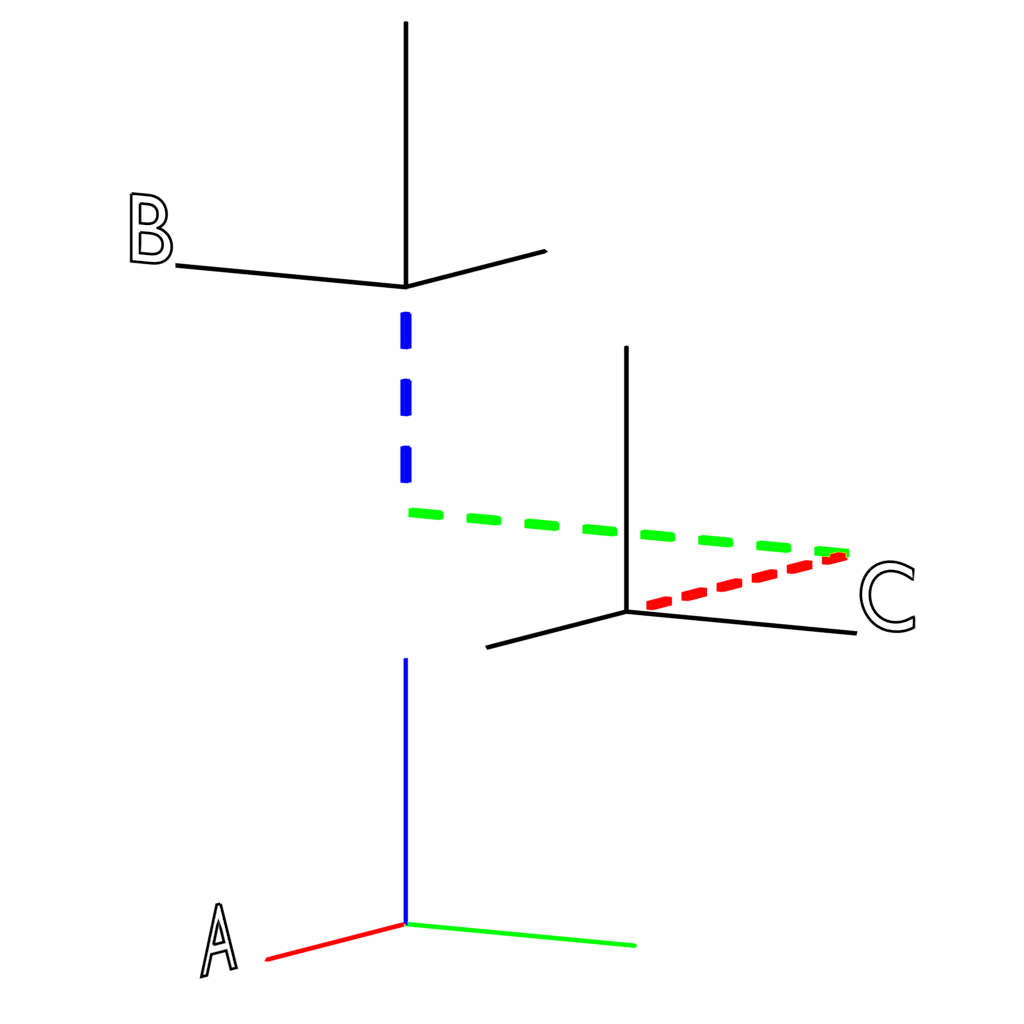
\includegraphics[width=0.5\textwidth]{Figures/Intro/FramesNC.png}
    \caption{Position Notation}
    \label{fig:position_notation}
\end{figure}
\end{definition}

\begin{definition}Let $^A\T_B$ denote the rotation matrix of frame $B$ frame A, with columns equating the basis vectors of $B$ measured in $A$.
\end{definition}

\begin{definition}Let $^A_B\omega_C$ denote the angular velocity of frame $C$ with respect to frame $B$, measured in frame $A$.
\end{definition}

\subsubsection{Rigid Bodies}

\begin{definition}
We define a link / rigid body $B$ as an tuple $B = \left (\B, \quad m_\B, \quad \BB\com, \quad \BB\J \right )$ where
\begin{align*}
    \B &:= \text{Frame of reference} \\
    m_\B &:= \text{Mass} \\
    \BB\com &:= \text{Center of Mass measured in/about $\B$} \\
    \BB\J &:= \text{Moment of inertia measured in/about $\B$} \\
\end{align*}
\begin{figure}[H]
    \centering
    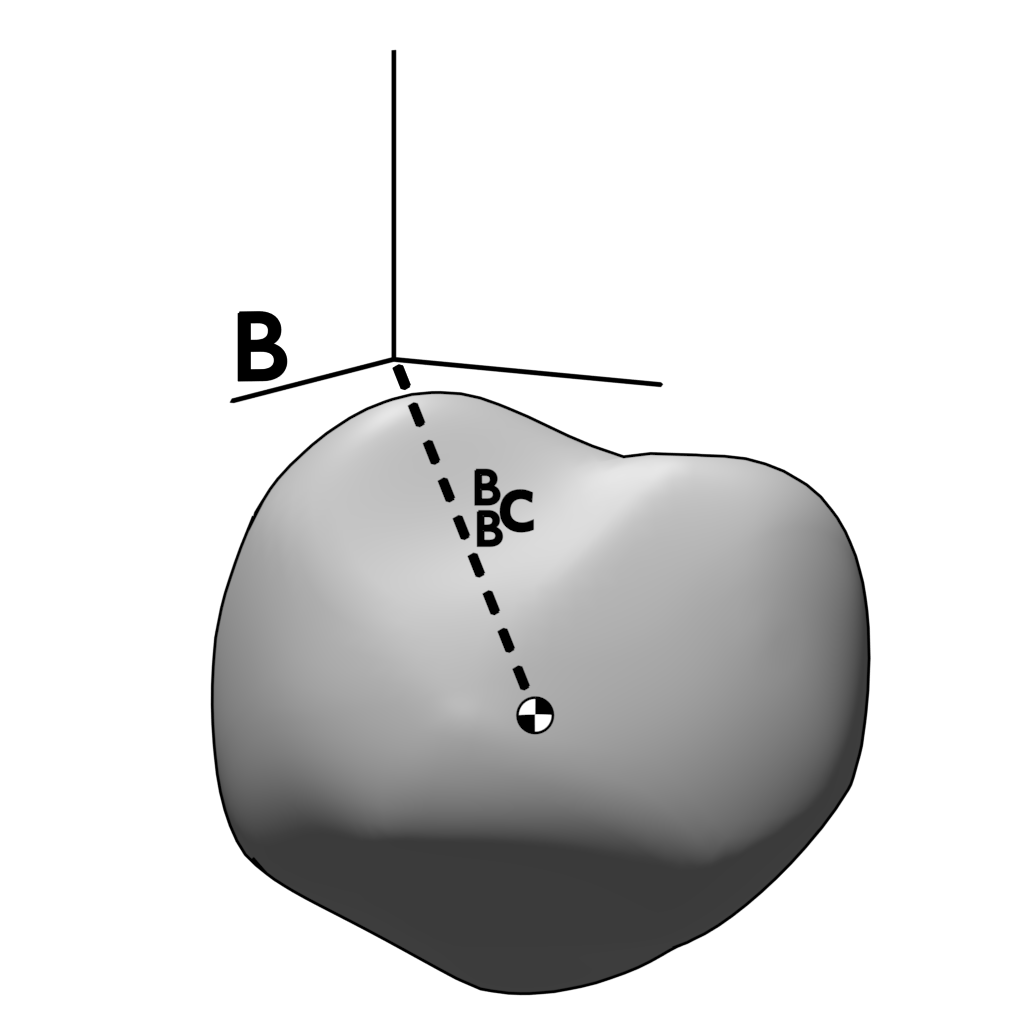
\includegraphics[width=0.5\textwidth]{Figures/Intro/BodyFrames.png}
    \caption{Body Notation}
    \label{fig:body_notation}
\end{figure}

\noindent References to a link/body and its frame of reference are used interchangeably throughout this text.
\end{definition}

\subsubsection{Joints}

\begin{definition}
A \textbf{prismatic joint} is a link that actuates on a linear axis.
\end{definition}

\begin{definition}
A \textbf{rotational joint} is a link that actuates on a rotating axis.
\end{definition}

\begin{definition}
An \textbf{open kinematic chain} is a series of connected links containing no closed loops.
\end{definition}


\begin{definition}Let $^A_B\r_C$ denote the position of frame $C$ with respect to frame $B$, measured in frame $A$.
\begin{figure}[H]
    \centering
    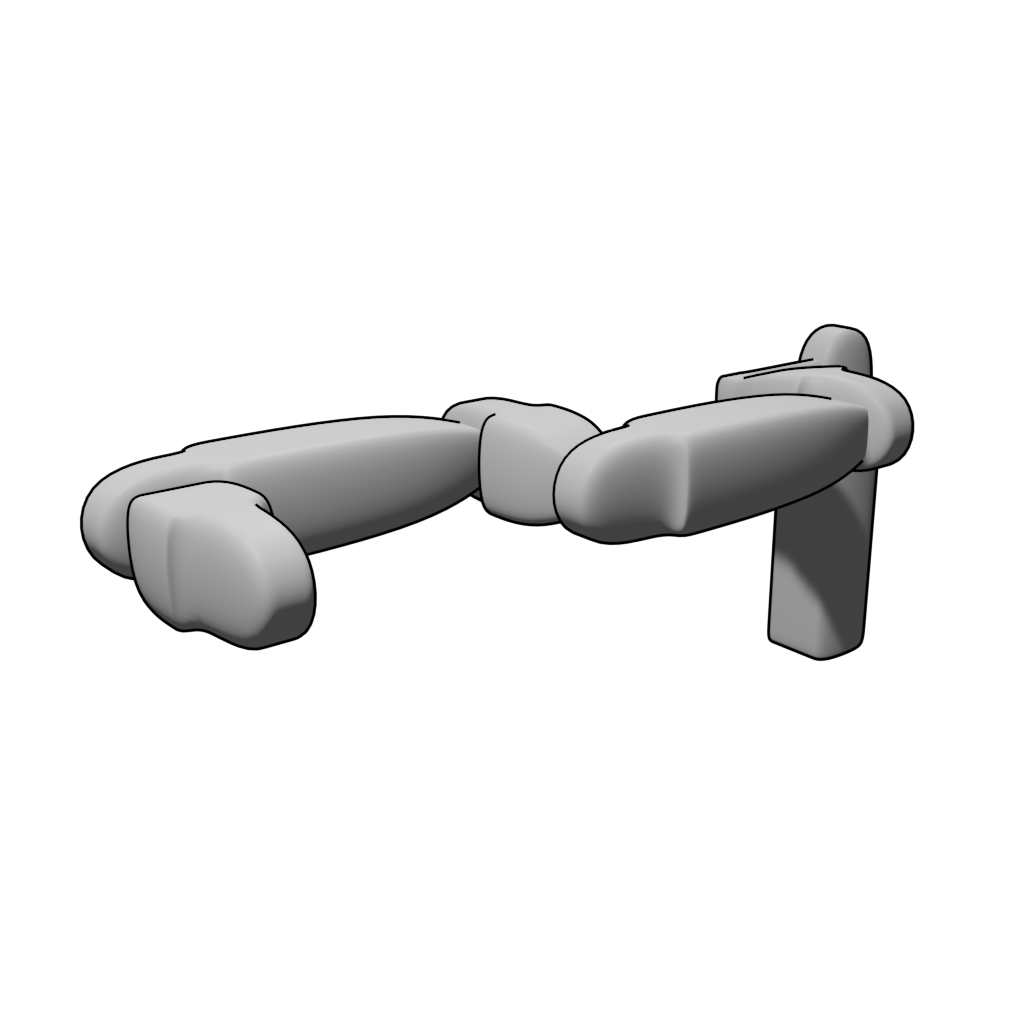
\includegraphics[width=0.4\textwidth]{Figures/Intro/OKC.png}
    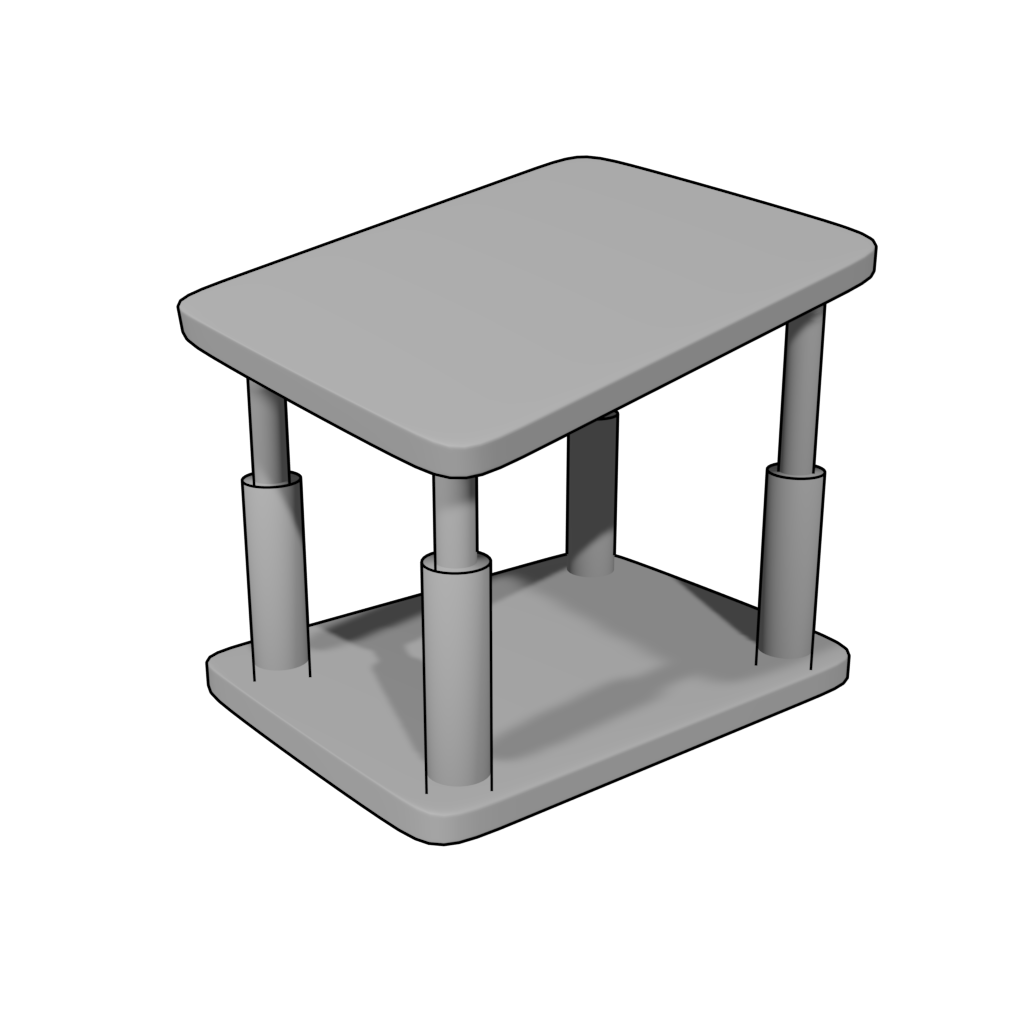
\includegraphics[width=0.4\textwidth]{Figures/Intro/NOKC.png}
    \caption{Open vs Closed Kinematic Chain}
    \label{fig:okc}
\end{figure}
\end{definition}


\begin{definition}
Let $B-1$ denote the link/body to which a link/body $B$ is attached in an open kinematic chain, off of which measurements are made.
\end{definition}

\section{The Newton Euler Formulation}

The Newton-Euler equations describe the translational and rotational motion of a rigid body through space \Cite{Hahn, asada_slotine_1986, shabana_2010}. Measured with respect to a coordinate frame at the center of mass of a body, 

\begin{align}
    \begin{bmatrix}
    \tau \\ \F
    \end{bmatrix} = 
    \begin{bmatrix}
     {\BB\J} & \ZERO_{3 \times 3} \\
      \ZERO_{3 \times 3} & m \EYE_{3 \times 3}
    \end{bmatrix}
    \begin{bmatrix}
     \mathbf{\dot{\omega}}\\
     \ddotx
    \end{bmatrix}
    + 
    \begin{bmatrix}
     \omega \times {\BB\J}\omega\\
     \ZERO_{3 \times 1} 
    \end{bmatrix}
\end{align}

\noindent Shifting the frame of reference, such that the center of mass is located at $\BB \com$, yields

\begin{align} \label{eqn:NE0}
    \begin{bmatrix}
    \tau \\ \F
    \end{bmatrix} = 
    \begin{bmatrix}
     {\BB\J} & m\S{\BB\com} \\
      -m\S{\BB\com} & m \EYE_{3 \times 3}
    \end{bmatrix}
    \begin{bmatrix}
     \ddotx\\
     \mathbf{\dot{\omega}}
    \end{bmatrix}
    + 
    \begin{bmatrix}
     \S{\omega}{\BB\J}\omega \\
     m \S{\omega}^2{\BB\com}
    \end{bmatrix}
\end{align}

%TODO: CHECK THIS CITATION TO MAKE SURE IT WORKS

\noindent Equation \ref{eqn:NE0} is limited to a single rigid body, however, it provides a starting point to model the motion of more complex systems. Such a model is given by the following equation \Cite{asada_slotine_1986, tedrake}, sometimes referred to as the \textit{Robot Equation} \Cite{isenberg_2020}.
\begin{align} \label{eqn:NE1}
    \H(\x)\ddotx = \F(\x, \dotx) - \d(\x, \dotx)
\end{align}

\noindent $\H$ is a positive definite $n \times n$ matrix, commonly called the System Mass Matrix \Cite{riley_hobson_bence_2006}. $\F$ contains external forces acting on the system, and $\d$ contains the Centrifugal and Coriolis forces, also called fictitious forces. Crucially, equation \ref{eqn:NE1} can be rewritten into a form that is Nonlinear Control Affine. \newline

A nonlinear control-affine system takes the following form
\begin{align} \label{eqn:NLCA}
    \dotx = \f(\x) + \g(\x) \u
\end{align}
\noindent Where $\x \in \mathbb{R}^n$ represents the state space configuration of the system, $\f$ denotes the natural response of the system, and $\g$ maps the control input $\u$ into the generalized coordinate space. $\ref{eqn:NE1}$ can be written into the form of \ref{eqn:NLCA}.
\begin{align*}
    \H \ddotx &= \F  - \d  \\ \nonumber
    \ddotx &= \H^{-1}\left (\F  - \d \right ) 
\end{align*}
\begin{align*} \nonumber
\text{Let  }  \X &= \begin{bmatrix} \x & \dotx \end{bmatrix}\transpose \\
    \dotX &= \begin{bmatrix}
     \dotx &\ddotx
    \end{bmatrix}\transpose 
    =
    \begin{bmatrix}
     \dotx \\ \H ^{-1}\left (\F  - \d \right ) 
    \end{bmatrix} 
    =
    \begin{bmatrix}
     \dotx \\ \H ^{-1}\left (\Fn  + \P\u - \d \right )
    \end{bmatrix} \\
    \text{where } \F &= \Fn  + \P(\x, \dotx)\u 
    \end{align*}
    \begin{align*}
    \dotX =
    \begin{bmatrix}
     \dotx \\ \H ^{-1}\left (\Fn  - \d \right ) + \H ^{-1}\left ( \P\u \right )
    \end{bmatrix} \\ &=
    \begin{bmatrix}
     \dotx \\ \H ^{-1}\left (\Fn  - \d \right )
    \end{bmatrix} + \begin{bmatrix}
     \ZERO_{n \times 1} \\  \H ^{-1} \P\u
    \end{bmatrix} \\
    &=
    \begin{bmatrix}
     \dotx \\ \H ^{-1}\left (\Fn  - \d \right )
    \end{bmatrix} + \begin{bmatrix}
     \ZERO_{n \times n} \\  \H ^{-1}\P
    \end{bmatrix}\u \\
    &= \f(\X) + \g(\X)\u \\
    \text{where } \f(\X) &= \begin{bmatrix}
     \dotx \\ \H ^{-1}\left (\Fn  - \d \right )
    \end{bmatrix} \\ \text{ and } \g(\X) &= \begin{bmatrix}
     \ZERO_{n \times n} \\  \H ^{-1}\P
    \end{bmatrix}
\end{align*}

% TODO: These equations are ugly. Fix the formatting.

\noindent With the system in control affine form allows for the usage of optimization-based controllers, such as Controller Barrier Functions (CBF).

\section{The CBF  - QP}

%TODO: Intro to this section
Control Barrier Functions provide an architecture for safety-aware controllers on nonlinear control affine systems \Cite{Ames1}. Such controllers operate by finding a control input that maintains invariance in the state of a system, $x \in \mathbb{R}^n$ with respect to a safe set, $C \in \mathbb{R}^n$. This safe safe set is represented in the controller through a \textit{barrier function}, $h(x) : \mathbb{R}^n \rightarrow \mathbb{R}$. We define $h(x)$ such that $C$ is a \textit{super-level set} of $h(x)$, yielding
\begin{align}
\begin{split}
    C = \left \{ x \in \mathbb{R}^n | h(x) \geq 0 \right \} 
\end{split}
\begin{split}
\end{split}
\begin{split}
    \partial C = \left \{ x \in \mathbb{R}^n | h(x) = 0 \right \}
\end{split}
\begin{split}
\end{split}
\begin{split}
    \text{Int}(C) = \left \{ x \in \mathbb{R}^n | h(x) > 0 \right \}
\end{split}
\end{align}

\noindent One can then prove safety for a system by showing $\dot{h}(x) \geq 0 \forall x \in \partial C$ \Cite{nagumo_1942}. In the case of nonlinear control affine systems, this is shown by
\begin{align}
    \Lie_f h(x) + \Lie_g h(x)u \geq -\alpha(h(x))
\end{align}
\noindent Where $\alpha(x)$ is a class $\kappa$ function, and $\Lie_p q$ denotes the \textit{Lie Derivative}, $\nabla q \cdot p$. \newline
This requirement can be expressed as a quadratic optimization problem, the goal of which is to find a control input that guarantees invariance of the safe set, shown in the following
\begin{align} \label{eqn:CBF-CLF-QP}
    u(x) = \argmin_{u \in \mathbb{R}^{m}} \quad &\frac{1}{2}(u - u_{ref}))^TH(x)(u - u_{ref})\\
    \textbf{s.t} \quad  &\Lie_f h(x) + \Lie_g h(x)u \geq -\alpha(h(x)) \nonumber
\end{align}

\noindent In this setting, $u_{ref}$ denotes the value of some reference controller on the system. In plain English, the goal of this quadratic program is to find the closest control input to $u_{ref}$ that satisfies the safety constraints of the system. In the case of min-norm controllers, $u_{ref}$ is set to 0. \newline

Note that the controller in Equation \ref{eqn:CBF-CLF-QP} is limited in that it is only applicable to first-order systems. That is systems in which the control input appears in the first derivative. Equation \ref{eqn:NE1} describes a second-order system, prohibiting the use of this controller. To implement a positional controller on these types of systems, High Order CBFs (HOCBF) must be used \Cite{Xiao, Nguyen}. \newline

The general constraint equation for a HOCBF is, 
\begin{align}
    \Lie_f^m h(x) + \Lie_g\Lie_f^{m-1}h(x)u + O(h(x)) + \alpha_m\left (\psi_{m-1}(x) \right ) \geq 0
\end{align}
\noindent Per Equation \ref{eqn:NE1}, $m = 2$, yielding
\begin{align}
   \begin{split}
        \psi_0(x) &= h(x) \\
        \psi_1(x) &= \dot{h}(x) + \alpha_1(h(x)))
   \end{split}
   \begin{split}
        \mathcal{C}_1 &= \{ x | \psi_0(x) \geq 0\} \\
        \mathcal{C}_2 &= \{ x | \psi_1(x) \geq 0\} \\
   \end{split}
\end{align}
\begin{align} \label{eqn:order2_cbf}
     \Lie_f^2 h(x) + \Lie_g\Lie_f h(x)u + \Lie_f h(x) + \alpha_2\left (\dot{h}(x) + \alpha_1(h(x))) \right ) \geq 0
\end{align}
Expanding the Lie derivatives in \ref{eqn:order2_cbf} yields
\begin{align}
    \Lie_f^2 h(x) + \Lie_g\Lie_f h(x)u &= \Lie_f (\nabla h(x) \cdot f(x)) + \Lie_g(\nabla h(x) \cdot f(x))u \nonumber\\
    &= \nabla (\nabla h(x) \cdot f(x)) \cdot f(x) + \nabla (\nabla h(x) \cdot f(x)) \cdot g(x) u \nonumber\\
    &= \nabla (\nabla h(x) \cdot f(x)) \cdot (f(x) + g(x)u) \nonumber\\
    &= (\nabla^2h(x)f(x) + h(x) \nabla f(x)) \cdot (f(x) + g(x)u) \label{eqn:lie_expanded}
\end{align}
\noindent where $\nabla^2h(x)$ denotes the Hessian matrix of $h$. \newline

Remember that $h(x)$ is a design choice, and can often be represented symbolically. This allows control designers to derive closed-form solutions for $\nabla h(x)$ and $\nabla^2 h(x)$ in advance, and optimize their online computation. The same is not necessarily true for $f(x)$ and $g(x)$. For many types of systems, open kinematic chains, these terms can grow exponentially in the number of degrees of freedom. This makes it infeasible to compute their value in real-time symbolically. Instead, algorithms were developed to compute their values numerically \Cite{isenberg_2020, walker_orin_1982}. This is sufficient for the evaluation of first-order CBFs, but second-order systems require the computation of $\nabla f(x)$, which cannot be solved from a numerical definition of $f$. To makes matters worse, the symbolic size of $\nabla f(x)$ is often even larger than $f(x)$, requiring $2n$ derivatives to be taken to account for the $n$ position and $n$ velocity dimensions in the state space. \newline

Existing works use approximations to combat the complexity of computing $\nabla f$, such as training neural networks to approximate CBF controllers \Cite{Yaghoubi}. While these significantly improve online performance, approximations by nature have weaker safety guarantees. Instead, I present a novel method of computing $\nabla f$ numerically, based on a technique for computing $f(x)$ introduced in \Cite{isenberg_2020}.

